\chapter{Anexo B: Manual de uso}
\label{ch:anexoc}

El objetivo de este apéndice es servir de guía para la ejecución del software diseñado, mostrar cómo es una partida del modo Jugador vs Máquina y mostrar los pasos a seguir para poner en marcha ambos modos.

Si bien el diseño del software está pensado para que resulte bastante intuitivo, se añade esta información para aclarar cualquier posible duda.


\section{Inicialización del algoritmo}

El primer paso es la inicialización del algoritmo necesaria para ejecutar los modos de juego \footnote{Solamente para los modos de juego en los que intervenga el algoritmo. Se puede ejecutar el modo Patrón vs Patrón sin necesidad de hacer este paso.}. Para ello, es necesario ejecutar un compilador de lenguaje R (el propio compilador de R instalado con la instalación de R en el equipo o otros más enfocados a la programación como RStudio) y cambiar el directorio de trabajo al directorio en que se encuentren todos los scripts del algoritmo. Tras esto, es necesario inicializar el sistema REST API. Para ello, tal y como se comentó en el apartado \ref{sec:APIrest}, se ejecutan los comandos necesarios:

\begin{verbatim}
source("inicializa.R")
inicializa()
r<-plumb("plumber.R")
r$run(port=8000).
\end{verbatim}

Cabe destacar que se utilizará el puerto 8000 para realizar la conexión con el API REST, y el motor de juego ha sido programado para leer desde ese puerto, por lo que si se decide cambiar el puerto, será necesario cambiar también el código del motor de juego.

Una vez arrancado el algoritmo, se puede arrancar el motor de juego, ejecutando el archivo \textit{Poker\_Simu.exe}, lo que abre una consola de comandos como la de la figura \ref{fig:C_ini}.

\begin{figure}[h]
\centering
\includegraphics[width=0.5\textwidth]{figuras/C_ini.png}   
\caption{Pantalla inicial de Poker\_Simu.exe}
\label{fig:C_ini}
\end{figure}

Tras esto, se elige la modalidad que se quiera jugar, escribiendo la letra J para el modo Jugador vs Máquina o M para el modo Máquina vs Máquina.

\section{Jugador Vs Máquina}

Una vez elegida esta modalidad, el propio juego te pedirá introducir la cantidad de dinero inicial para los jugadores y el valor de la Ciega Grande, tal como se muestra en la imagen \ref{fig:C_ji}.

\begin{figure}[h]
\centering
\includegraphics[width=0.5\textwidth]{figuras/C_ji.png}   
\caption{Pantalla inicial de Poker\_Simu.exe en el modo Jugador vs Máquina.}
\label{fig:C_ji}
\end{figure}

Una vez introducidos, se comenzará la partida, mostrando la mesa disponible para el jugador. Es decir, mostrará las cartas de la mano del jugador. Tras esto, comenzará el juego. Cada vez que sea el turno del jugador, siguiendo el flujo de juego. Este proceso se irá repitiendo hasta que uno pase o ambos vean la apuesta.
Una vez que se pase al preflop, mostrará las cartas de la mesa, tal y como aparece en la imagen \ref{fig:C_j2}.

\begin{figure}[h]
\centering
\includegraphics[width=0.5\textwidth]{figuras/C_j2.png}   
\caption{Flop en el modo Jugador vs Máquina.}
\label{fig:C_j2}
\end{figure}


\begin{figure}[h]
\centering
\includegraphics[width=0.5\textwidth]{figuras/C_JE.png}   
\caption{Subida de apuesta en el modo Jugador vs Máquina.}
\label{fig:C_JE}
\end{figure}

\begin{figure}[h]
\centering
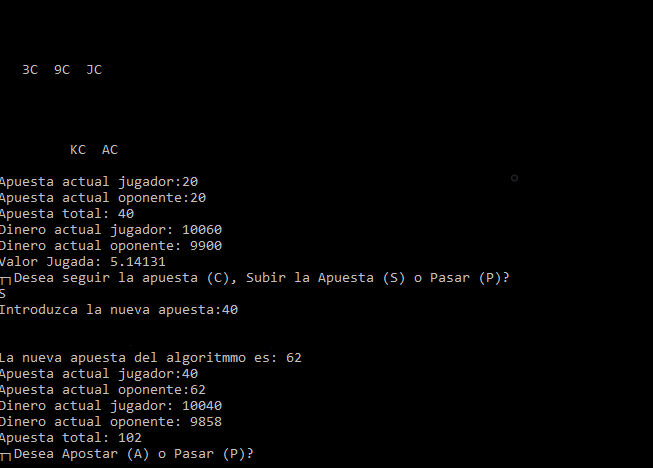
\includegraphics[width=0.5\textwidth]{figuras/C_J.png}   
\caption{Reacción del algoritmo ante una acción del jugador.}
\label{fig:C_J}
\end{figure}

En caso de hacer una subida, se pedirá que se introduzca la cantidad a subir, como aparece en \ref{fig:C_JE}. En caso de que el algoritmo tome una decisión, esta acción será mostrada y pedirá al jugador que tome una acción en caso de que sea necesario, tal como aparece en \ref{fig:C_J}.

\begin{figure}[h]
\centering
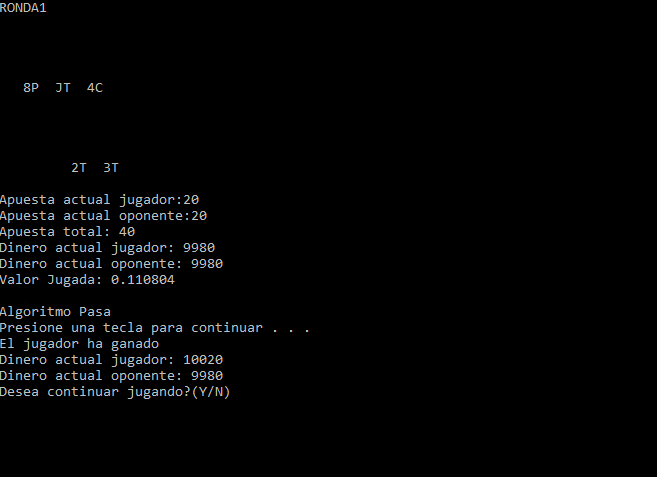
\includegraphics[width=0.5\textwidth]{figuras/C_jf.png}   
\caption{Fin de ronda.}
\label{fig:C_jf}
\end{figure}

Una vez que uno de los jugadores pase, o se llegue al showdown y se acabe la ronda de apuestas, se pedirá al jugador si quiere seguir jugando, a lo que tendrá que responder escribiendo Y en caso de que se quiera seguir jugando, o N en caso de querer acabar la partida. (Tal como se muestra en \ref{fig:C_jf}.)

\clearpage

\section{Máquina Vs Máquina}

En este apartado, se muestra cómo se desarrolla el juego en caso de haber elegido el modo Máquina vs Máquina. Una vez introducida la opción, se listarán los 3 patrones posibles (Maniaco, Roca y Calling Station), tras lo cual se pide al jugador introducir que modo dentro del modo Máquina vs Máquina. Tal como se muestra en la figura

\begin{figure}[h]
\centering
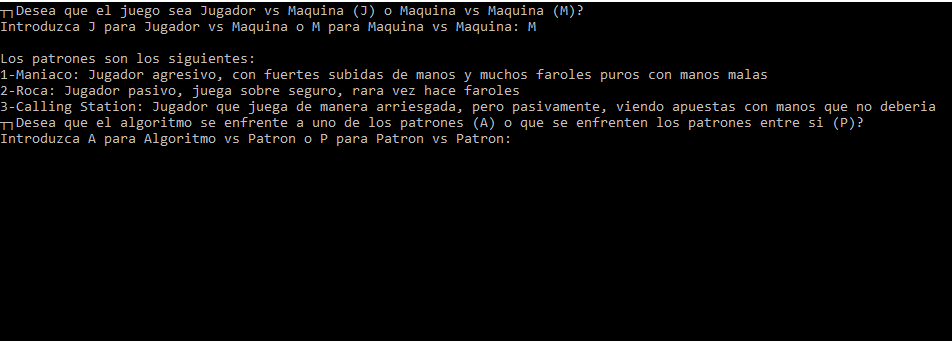
\includegraphics[width=0.5\textwidth]{figuras/C_M.png}   
\caption{Pantalla de inicio del modo Máquina vs Máquina.}
\label{fig:C_M}
\end{figure}

En caso de que se elija el modo Patrón vs Patrón, se mostrarán las tres combinaciones (Maniaco vs Roca, Roca vs Calling Station y Calling Station vs Maniaco) y después pide al jugador que introduzca la combinación de patrones que quiere que se enfrenten (como aparece en la imagen \ref{fig:C_MM}) . En caso de que se elija el modo Algoritmo vs Patrón, se pedirá al jugador que introduzca a cual de los 3 patrones desea que se enfrente al algoritmo (como se muestra en la imagen \ref{fig:C_MA}). Tras eso se pide al jugador que introduzca el dinero inicial de cada jugador, así como el valor de la Ciega Grande. Por último, se pide introducir el número de interacciones deseadas.

\begin{figure}[h]
\centering
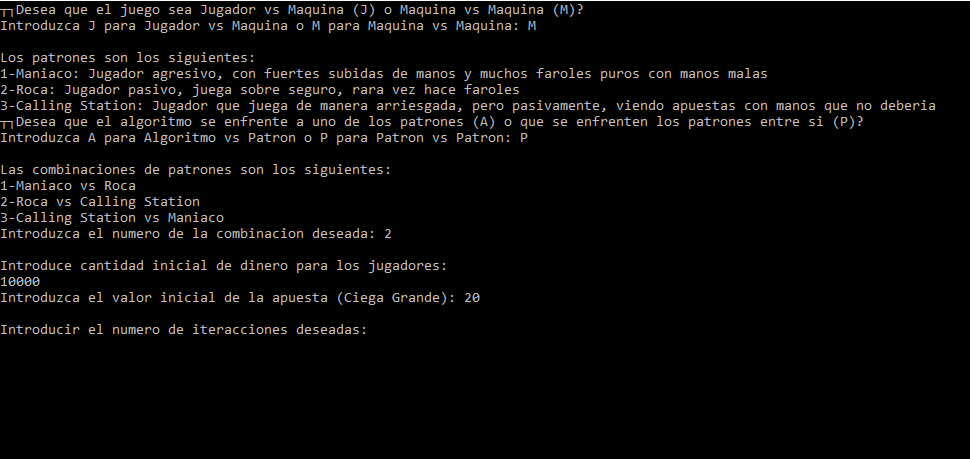
\includegraphics[width=0.5\textwidth]{figuras/C_MM.png}   
\caption{Pantalla de inicio del modo Patrón vs Patrón.}
\label{fig:C_MM}
\end{figure}

\begin{figure}[h]
\centering
\includegraphics[width=0.5\textwidth]{figuras/C_MA.png}   
\caption{Pantalla de inicio del modo Algoritmo vs Patron..}
\label{fig:C_MA}
\end{figure}

Estas iteracciones se irán ejecutando sin necesidad de intervención por parte del jugador. Una vez se alcance una de las condiciones de fin de juego (se alcance el número de iteraciones o uno de los jugadores se quede sin dinero), finalizará el programa. El resultado de las iteraciones se almacenará en un fichero .txt, con un formato como el que se mostró \ref{fig:resultados}.